\newpage

\section{Moments d'une distribution}

\subsection{Définitions fondamentales des moments}

\begin{definitionbox}[Types de Moments]
Soit $X$ une variable aléatoire ayant une espérance $\mu$ et une variance $\sigma^2$. Pour tout entier positif $m$, on définit les moments suivants :
\begin{itemize}
    \item \textbf{$m$-ième moment (non centré)} : $E[X^m]$.
    \item \textbf{$m$-ième moment centré} : $E[(X - \mu)^m]$.
    \item \textbf{$m$-ième moment standardisé} : $E\left[\left(\frac{X - \mu}{\sigma}\right)^m\right]$.
\end{itemize}
Les moments centrés et standardisés permettent d'étudier les propriétés de la distribution indépendamment de sa position ($\mu$) et de son échelle ($\sigma$).
\end{definitionbox}

\subsection{Asymétrie (Skewness)}

\begin{definitionbox}[Asymétrie (Skewness)]
L'\textbf{asymétrie} (ou \textit{skewness}) d'une variable aléatoire $X$ de moyenne $\mu$ et d'écart-type $\sigma$ est définie comme le \textbf{troisième moment standardisé} :
$$ \text{Skew}(X) = E\left[ \left( \frac{X - \mu}{\sigma} \right)^3 \right]. $$
\end{definitionbox}

\begin{intuitionbox}[Comprendre la Formule du Skewness]
Pour une variable aléatoire $X$ de moyenne $\mu$ et d'écart-type $\sigma$, le \textbf{skewness} est défini comme :
\[
\text{Skew}(X) = \frac{E[(X - \mu)^3]}{\sigma^3}
\]

\medskip

\textbf{Logique du numérateur : le moment centré d'ordre 3}
\begin{itemize}
    \item Le terme $(X - \mu)^3$ est le \textbf{cube de l'écart à la moyenne}
    \item Contrairement à $(X - \mu)^2$ (toujours positif), le cube \textbf{conserve le signe} de l'écart
    \item Il pondère différemment les observations à gauche et à droite de la moyenne
\end{itemize}

\medskip

\textbf{Interprétation intuitive}
\begin{itemize}
    \item \textbf{Skewness = 0} : Distribution symétrique, écarts positifs et négatifs s'annulent
    \item \textbf{Skewness > 0} : Queue longue à droite, grandes valeurs positives amplifiées par le cube
    \item \textbf{Skewness < 0} : Queue longue à gauche, écarts négatifs dominent
\end{itemize}

\medskip

\textbf{Pourquoi $\sigma^3$ au dénominateur ?}
\begin{itemize}
    \item Le moment d'ordre 3 est homogène à des unités au cube
    \item On divise par $\sigma^3$ pour obtenir un coefficient \textbf{sans dimension}
    \item Permet la comparaison entre distributions de différentes échelles
\end{itemize}

\begin{center}
\begin{tabular}{|c|c|c|}
\hline
\textbf{Type} & \textbf{Forme} & \textbf{Interprétation} \\
\hline
$\text{Skew} = 0$ & Symétrique & Moyenne = Médiane = Mode \\
\hline
$\text{Skew} > 0$ & Queue à droite & Valeurs extrêmes tirent la moyenne vers la droite \\
\hline
$\text{Skew} < 0$ & Queue à gauche & Valeurs extrêmes tirent la moyenne vers la gauche \\
\hline
\end{tabular}
\end{center}
\end{intuitionbox}

\begin{remarquebox}[Pourquoi Standardiser ?]
En standardisant d'abord ($\frac{X-\mu}{\sigma}$), la définition de $\text{Skew}(X)$ ne dépend ni de la position ($\mu$) ni de l'échelle ($\sigma$) de la distribution, ce qui est raisonnable puisque ces informations sont déjà fournies par la moyenne et l'écart-type. De plus, cette standardisation garantit que l'asymétrie est invariante par changement d'unité de mesure (par exemple, passer des pouces aux mètres n'affecte pas la valeur de l'asymétrie).
\end{remarquebox}

\subsection{Propriétés de symétrie}

\begin{definitionbox}[Symétrie d'une Variable Aléatoire]
On dit qu'une variable aléatoire $X$ a une distribution \textbf{symétrique} autour de $\mu$ si la variable $X - \mu$ a la même distribution que $\mu - X$. On dit aussi que $X$ est symétrique ou que sa distribution est symétrique. Ces trois formulations ont le même sens.
\end{definitionbox}

\begin{theorembox}[Symétrie en Termes de Fonction de Densité]
Soit $X$ une variable aléatoire continue de fonction de densité de probabilité (PDF) $f$. Alors, $X$ est symétrique autour de $\mu$ si et seulement si :
$$ f(x) = f(2\mu - x) \quad \text{pour tout } x. $$
\end{theorembox}

\begin{proofbox}[Preuve du Théorème de Symétrie]
Soit $F$ la fonction de répartition (CDF) de $X$. Si la symétrie tient, alors :
$$ F(x) = P(X \le x) = P(X - \mu \le x - \mu) = P(\mu - X \le x - \mu) = P(X \ge 2\mu - x) = 1 - F(2\mu - x). $$

En prenant la dérivée des deux côtés par rapport à $x$, on obtient :
$$ f(x) = \frac{d}{dx}F(x) = \frac{d}{dx}[1 - F(2\mu - x)] = f(2\mu - x). $$

Cela démontre que la condition $f(x) = f(2\mu - x)$ est nécessaire et suffisante pour la symétrie.
\end{proofbox}

\subsection{Aplatissement (Kurtosis)}

\begin{definitionbox}[Kurtosis (Aplatissement)]
Pour une variable aléatoire $X$ de moyenne $\mu$ et d'écart-type $\sigma$, le \textbf{kurtosis} est défini comme le \textbf{quatrième moment standardisé} :
$$ \text{Kurtosis}(X) = E\left[ \left( \frac{X - \mu}{\sigma} \right)^4 \right]. $$

Dans la pratique, on utilise plus souvent le \textbf{kurtosis excessif} (ou excès de kurtosis), défini comme :
$$ \text{Excess Kurtosis}(X) = E\left[ \left( \frac{X - \mu}{\sigma} \right)^4 \right] - 3. $$
La soustraction de 3 fait en sorte que le kurtosis d'une loi normale soit égal à 0.
\end{definitionbox}

\begin{intuitionbox}[Comprendre la Kurtosis]
Pour une variable aléatoire $X$, le \textbf{kurtosis} est défini comme :
\[
\text{Kurt}(X) = \frac{E[(X - \mu)^4]}{\sigma^4}
\]
et l'\textbf{excess kurtosis} (kurtosis excédentaire) comme : $\text{Excess Kurtosis} = \text{Kurt}(X) - 3$.

\medskip

\textbf{Pourquoi le moment d'ordre 4 ?}
\begin{itemize}
    \item Comme la variance, on utilise une puissance paire (pas d'effet de signe)
    \item La puissance 4 \textbf{amplifie énormément les écarts extrêmes}
    \item Mesure le \textbf{poids des queues} et la \textbf{concentration autour de la moyenne}
\end{itemize}

\medskip

\textbf{Interprétation intuitive}
\begin{itemize}
    \item \textbf{Excess Kurtosis = 0} (Kurtosis = 3) : Distribution normale (mésocurtique)
    \item \textbf{Excess Kurtosis < 0} (Kurtosis < 3) : Distribution aplatie (platykurtique) — queues légères
    \item \textbf{Excess Kurtosis > 0} (Kurtosis > 3) : Distribution pointue avec queues épaisses (leptokurtique)
\end{itemize}

\medskip

\textbf{Application en finance}
\begin{itemize}
    \item Les rendements financiers ont souvent un excès de kurtosis positif
    \item Indique une probabilité plus élevée d'événements extrêmes que la loi normale
    \item Justifie le "vol smile" dans les options
\end{itemize}

\medskip

\textbf{Pourquoi $\sigma^4$ au dénominateur ?}
\begin{itemize}
    \item Le moment d'ordre 4 est homogène à des unités$^4$
    \item On divise par $\sigma^4$ pour un coefficient \textbf{sans dimension}
\end{itemize}

\begin{center}
\begin{tabular}{|c|c|c|c|}
\hline
\textbf{Type} & \textbf{Kurtosis} & \textbf{Excess} & \textbf{Caractéristiques} \\
\hline
Platykurtique & $< 3$ & $< 0$ & Queues légères, centre large \\
\hline
Mésocurtique & $= 3$ & $= 0$ & Référence normale \\
\hline
Leptokurtique & $> 3$ & $> 0$ & Queues épaisses, pic pointu \\
\hline
\end{tabular}
\end{center}
\end{intuitionbox}

\subsection{Exemples de distributions}

\begin{examplebox}[La Distribution Normale (Mésokurtique)]

\begin{center}
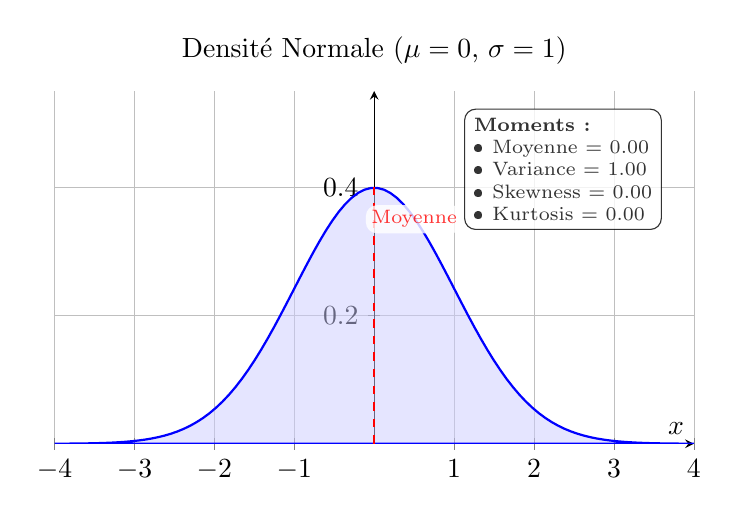
\begin{tikzpicture}
  \begin{axis}[
    width=0.8\textwidth,
    height=0.5\textwidth,
    xlabel={$x$},
    title={Densité Normale ($\mu=0$, $\sigma=1$)},
    grid=both,
    grid style={line width=.1pt, draw=gray!30},
    major grid style={line width=.2pt,draw=gray!50},
    domain=-4:4,
    samples=100,
    enlargelimits=false,
    axis lines=middle,
    xmin=-4, xmax=4,
    ymin=0, ymax=0.55
  ]
  
  % Courbe de densité
  \addplot [thick, color=blue, fill=blue!20, fill opacity=0.5] 
    {1/(sqrt(2*pi))*exp(-x^2/2)} \closedcycle;
  
  % Ligne de la moyenne
  \addplot [red, dashed, thick] coordinates {(0,0) (0,0.4)};
  \node[red, fill=white, font=\scriptsize, rounded corners, inner sep=2pt, opacity=0.8] at (axis cs:0.5,0.35) {Moyenne};
  
  % Boîte de texte avec moments seulement
  \node [draw=black, fill=white, rounded corners, font=\scriptsize, align=left, anchor=north east, opacity=0.8] 
    at (axis description cs:0.95,0.95) { % MODIFIÉ
    \textbf{Moments :}\\
    • Moyenne = 0.00\\
    • Variance = 1.00\\
    • Skewness = 0.00\\
    • Kurtosis = 0.00
    };
    
  \end{axis}
\end{tikzpicture}
\end{center}

La distribution normale est l'archétype de la courbe en cloche. Imaginez une cible : la majorité des flèches touchent le centre, et plus on s'éloigne du centre, moins il y a de chances d'être touché. C'est une distribution parfaitement symétrique, ce qui se traduit par un \textbf{skewness nul (0.00)}. Son pic est ni trop pointu, ni trop plat : c'est notre point de référence, on dit qu'elle est \textbf{mésokurtique}, d'où son kurtosis de \textbf{0.00}. C'est la base de nombreuses analyses statistiques car elle modélise naturellement beaucoup de phénomènes.

\end{examplebox}

\begin{examplebox}[La Distribution Exponentielle (Asymétrique à Droite)]

\begin{center}
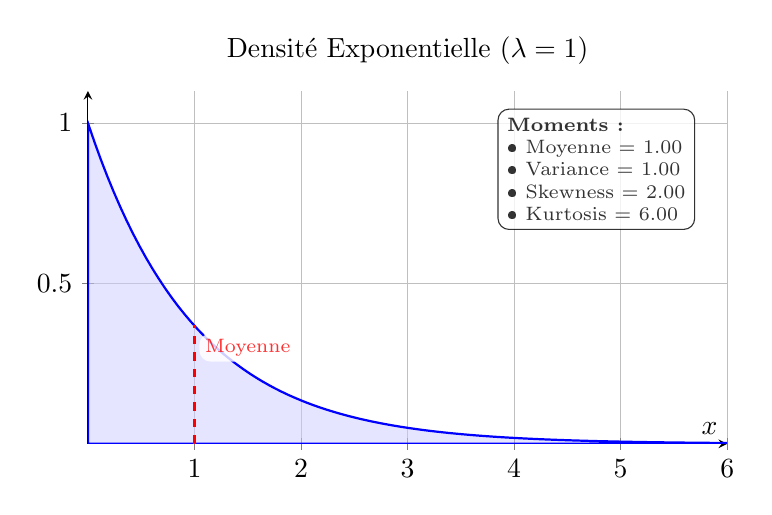
\begin{tikzpicture}
  \begin{axis}[
    width=0.8\textwidth,
    height=0.5\textwidth,
    xlabel={$x$},
    title={Densité Exponentielle ($\lambda=1$)},
    grid=both,
    grid style={line width=.1pt, draw=gray!30},
    major grid style={line width=.2pt,draw=gray!50},
    domain=0:6,
    samples=100,
    enlargelimits=false,
    axis lines=middle,
    xmin=0, xmax=6,
    ymin=0, ymax=1.1
  ]
  
  % Courbe de densité exponentielle
  \addplot [thick, color=blue, fill=blue!20, fill opacity=0.5] 
    {exp(-x)} \closedcycle;
  
  % Ligne de la moyenne
  \addplot [red, dashed, thick] coordinates {(1,0) (1,0.37)};
  \node[red, fill=white, font=\scriptsize, rounded corners, inner sep=2pt, opacity=0.8] at (axis cs:1.5,0.3) {Moyenne};
  
  % Boîte de texte avec moments seulement
  \node [draw=black, fill=white, rounded corners, font=\scriptsize, align=left, anchor=north east, opacity=0.8] 
    at (axis description cs:0.95,0.95) { % MODIFIÉ
    \textbf{Moments :}\\
    • Moyenne = 1.00\\
    • Variance = 1.00\\
    • Skewness = 2.00\\
    • Kurtosis = 6.00
    };
    
  \end{axis}
\end{tikzpicture}
\end{center}

Imaginez le temps d'attente avant un événement rare, comme un appel téléphonique. La plupart du temps, l'appel arrive vite, mais il peut parfois y avoir de longues attentes. C'est exactement ce que modélise la distribution exponentielle : un pic à gauche et une longue queue à droite. Cela se traduit par un \textbf{skewness positif élevé (2.00)}, indiquant une asymétrie marquée. Elle est aussi \textbf{leptokurtique} (\textbf{kurtosis = 6.00}) : son pic est pointu, et la longue queue droite signifie qu'il y a une probabilité non négligeable de valeurs extrêmes.

\end{examplebox}

\begin{examplebox}[La Distribution Uniforme (Platykurtique)]

\begin{center}
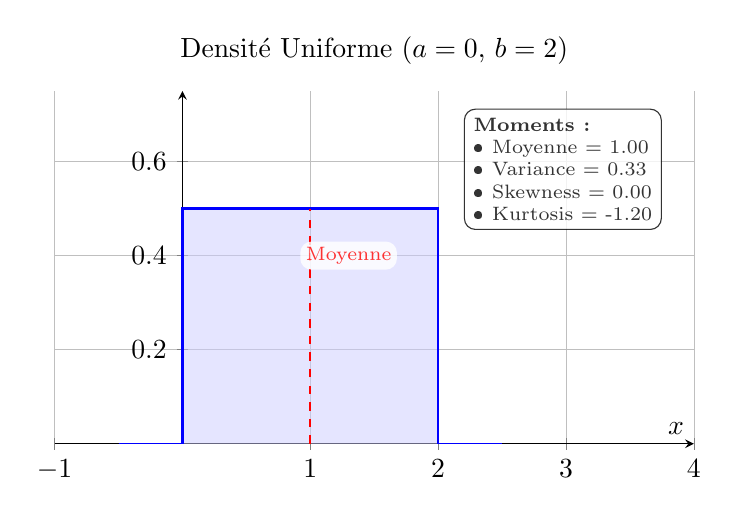
\begin{tikzpicture}
  \begin{axis}[
    width=0.8\textwidth,
    height=0.5\textwidth,
    xlabel={$x$},
    title={Densité Uniforme ($a=0$, $b=2$)},
    grid=both,
    grid style={line width=.1pt, draw=gray!30},
    major grid style={line width=.2pt,draw=gray!50},
    domain=-0.5:2.5,
    samples=100,
    enlargelimits=false,
    axis lines=middle,
    ymin=0,
    ymax=.75,
    xmin=-1, xmax=4
  ]
  
  % Courbe de densité uniforme
  \addplot [thick, color=blue, fill=blue!20, fill opacity=0.5, const plot] 
    coordinates {(-0.5,0) (0,0) (0,0.5) (2,0.5) (2,0) (2.5,0)};
  
  % Ligne de la moyenne
  \addplot [red, dashed, thick] coordinates {(1,0) (1,0.5)};
  \node[red, fill=white, font=\scriptsize, rounded corners, inner sep=2pt, opacity=0.8] at (axis cs:1.3,0.4) {Moyenne};
  
  % Boîte de texte avec moments seulement
  \node [draw=black, fill=white, rounded corners, font=\scriptsize, align=left, anchor=north east, opacity=0.8] 
    at (axis description cs:0.95,0.95) { % MODIFIÉ
    \textbf{Moments :}\\
    • Moyenne = 1.00\\
    • Variance = 0.33\\
    • Skewness = 0.00\\
    • Kurtosis = -1.20
    };
    
  \end{axis}
\end{tikzpicture}
\end{center}

La distribution uniforme, c'est le "tirage au sort parfait" : chaque valeur sur un intervalle a la même chance d'être tirée. Visuellement, c'est un rectangle, donc aucune valeur n'est privilégiée. Elle est symétrique (\textbf{skewness = 0.00}), mais contrairement à la normale, elle est "plate", sans pic central. Cela se traduit par un \textbf{kurtosis négatif (-1.20)}, ce qui signifie qu'elle est \textbf{platykurtique}. Elle est donc très différente des distributions avec un pic central comme la normale.

\end{examplebox}

\begin{examplebox}[La Distribution Log-Normale (Fortement Leptokurtique)]

\begin{center}
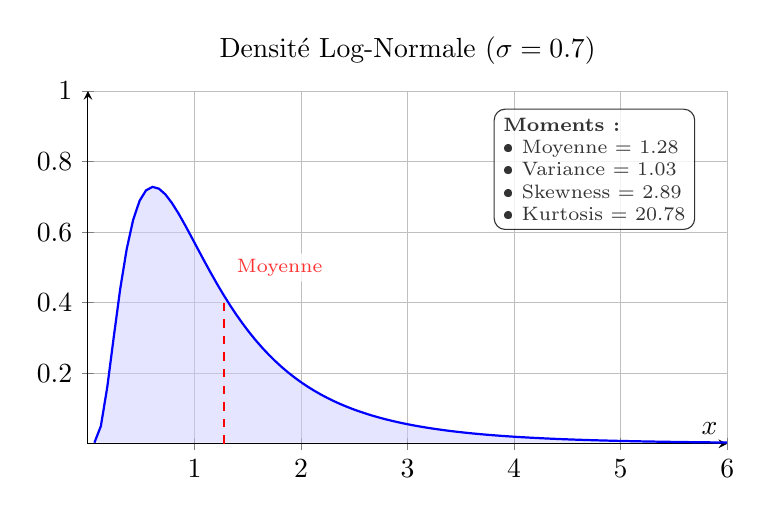
\begin{tikzpicture}
  \begin{axis}[
    width=0.8\textwidth,
    height=0.5\textwidth,
    xlabel={$x$},
    title={Densité Log-Normale ($\sigma=0.7$)},
    grid=both,
    grid style={line width=.1pt, draw=gray!30},
    major grid style={line width=.2pt,draw=gray!50},
    domain=0:6,
    samples=100,
    enlargelimits=false,
    axis lines=middle,
    xmin=0, xmax=6,
    ymin=0, ymax=1
  ]
  
  % Courbe de densité log-normale
  \addplot [thick, color=blue, fill=blue!20, fill opacity=0.5] 
    {1/(x*0.7*sqrt(2*pi))*exp(-(ln(x))^2/(2*0.7^2))};
  
  % Ligne de la moyenne
  \addplot [red, dashed, thick] coordinates {(1.28,0) (1.28,0.4)};
  \node[red, fill=white, font=\scriptsize, rounded corners, inner sep=2pt, opacity=0.8] at (axis cs:1.8,0.5) {Moyenne};
  
  % Boîte de texte avec moments seulement
  \node [draw=black, fill=white, rounded corners, font=\scriptsize, align=left, anchor=north east, opacity=0.8] 
    at (axis description cs:0.95,0.95) { % MODIFIÉ
    \textbf{Moments :}\\
    • Moyenne = 1.28\\
    • Variance = 1.03\\
    • Skewness = 2.89\\
    • Kurtosis = 20.78
    };
    
  \end{axis}
\end{tikzpicture}
\end{center}

La log-normale est une distribution très asymétrique. Imaginez la richesse d'une population : la majorité est modeste, mais il existe une petite proportion de très riches, ce qui "étire" la droite de la courbe. Cela donne un \textbf{skewness très élevé (2.89)}. Elle est extrêmement \textbf{leptokurtique} (\textbf{kurtosis = 20.78}) : un pic très aigu et une queue droite très lourde. Cela signifie qu'il y a un risque élevé de valeurs extrêmement grandes, ce qui la rend très utile pour modéliser des phénomènes avec de rares événements extrêmes.

\end{examplebox}